\documentclass{beamer}

\usepackage[ngerman]{babel}
\usepackage[utf8]{inputenc}
\usepackage[T1]{fontenc}
\usepackage{lmodern}
\usepackage{pdfpages}

\usetheme{Boadilla}  %% Themenwahl
\usecolortheme{whale}


%% Variables. You may want to change them. 
\title{Campusrally Siegerehrung}
\subtitle{Fachschaft MPI}
\author{}
\date{\today}

\setbeamertemplate{headline}
{
  \leavevmode%
  \hbox{%
  \begin{beamercolorbox}[wd=\paperwidth,ht=8.25ex,dp=1.5ex]{palette secondary}
    \raggedright
    \hspace*{2em}%
    
\includegraphics[width=15mm]{media/fachschaft.png} 
    \hspace{100pt}
\includegraphics[width=5mm]{media/fakultaet_mathe.png}
    \hspace{10pt}
\includegraphics[width=5mm]{media/fakultaet_physik.png}
    \hspace{10pt}
\includegraphics[width=5mm]{media/fakultaet_informatik.png}
    \hspace{100pt}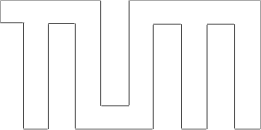
\includegraphics[width=10mm]{media/tum.png}
    \hspace*{2em}%
  \end{beamercolorbox}%
  }%
}


% If you want to get rid of the presentation controls in the bottom right corner, enable this setting
% \setbeamertemplate{navigation symbols}{} 

% This setting removes the footer but keeps the frame (=slide) number in the bottom right corner
% \setbeamertemplate{footline}[frame number]{}

% This setting removes the footer completely. It is going to override footer-related settings from above!
% \setbeamertemplate{footline}{}

%%%%%%%%%%%%%%%%%%%%%%%%%%%%%%%%%%%%%%%%%%%%%%%%%%%%%%%%%%%%%%%%%%%%%%%%%%%%%%%%%%%%%%%%%%%%%%%%%%%%%%%%%%%%%%%%%%%%%%%
% The content starts here
\begin{document}



% First page
\maketitle
% Comment this out to remove the table of contents


\begin{frame}
\huge
\center
1. Platz:
\\
\ \\
Gruppe 22
\\
Masters of Desasters
\\
127 Punkte
\end{frame}

\begin{frame}
\huge
\center
2. Platz:
\\
\ \\
Gruppe 1
\\
\
\\
116 Punkte
\end{frame}

\begin{frame}
\huge
\center
3. Platz:
\\
\ \\
Gruppe 25
\\
Kein Bier vor 4!
\\
114 Punkte
\end{frame}

\begin{frame}
\huge
\center
4. Platz:
\\
\ \\
Gruppe 29
\\
Die glorreichen 7 1/2
\\
110 Punkte
\end{frame}

\begin{frame}
\huge
\center
5. Platz:
\\
\ \\
Gruppe 28
\\
Hello World!
\\
105 Punkte
\end{frame}

\begin{frame}
\huge
\center
6. Platz:
\\
\ \\
Gruppe 15
\\
Atomindustrie
\\
104 Punkte
\end{frame}

\begin{frame}
\huge
\center
7. Platz:
\\
\ \\
Gruppe 1900
\\
MCM
\\
99 Punkte
\end{frame}

\begin{frame}
\huge
\center
8. Platz:
\\
\ \\
Gruppe 12
\\
); DROP TABLE "Gruppen";
\\
99 Punkte
\end{frame}

\begin{frame}
\huge
\center
9. Platz:
\\
\ \\
Gruppe 1400
\\
Sieger
\\
95 Punkte
\end{frame}

\begin{frame}
\huge
\center
10. Platz:
\\
\ \\
Gruppe 200
\\
\
\\
94 Punkte
\end{frame}

\begin{frame}
\huge
\center
11. Platz:
\\
\ \\
Gruppe 2
\\
SMOTMA
\\
94 Punkte
\end{frame}

\begin{frame}
\huge
\center
12. Platz:
\\
\ \\
Gruppe 1500
\\
1500
\\
90 Punkte
\end{frame}

\begin{frame}
\huge
\center
13. Platz:
\\
\ \\
Gruppe 8
\\
\
\\
90 Punkte
\end{frame}
%Diagramm über den Fakt, dass Übung sehr wichtig ist?!

% Sections are like chapters and used to structure the presentation 

\end{document}
